\documentclass[11pt]{article}

\usepackage{deauthor}
\usepackage{times}
\usepackage{graphicx}
\graphicspath{{figs/}}


\title{Plenario}
\author{Charlie Catlett, Jonathan Giuffrida, Brett Goldstein, Robert Mitchum\footnote{The Plenario project is funded by the John D. and Catherine T. MacArthur Foundation and the National Science Foundation via an NSF Early-Concept Grant for Exploratory Research (EAGER) for software development (award number 1348865), while the interaction capabilities were driven by the Urban Sciences Research Coordination Network, created with an NSF Building Community and Capacity for Data-Intensive Research in the Social, Behavioral, and Economic Sciences and in Education and Human Resources (BCC-SBE/EHR) award. \newline \newline All authors: The Urban Center for Computation and Data (http://urbanccd.org). Catlett: Argonne National Laboratory (http://anl.gov). Catlett and Mitchum: The Computation Institute (http://ci.uchicago.edu). Giuffrida and Goldstein: The Harris School for Public Policy Studies, The University of Chicago (http://harris.uchicago.edu).}}
\date{Submitted January, 2015}
\begin{document}
\maketitle 


\begin{abstract}

\end{abstract}

\section{Introduction and Landscape}

\section{Platform}
\begin{figure}[h]
	\caption{Dataset Lifecycle}
	\centering
	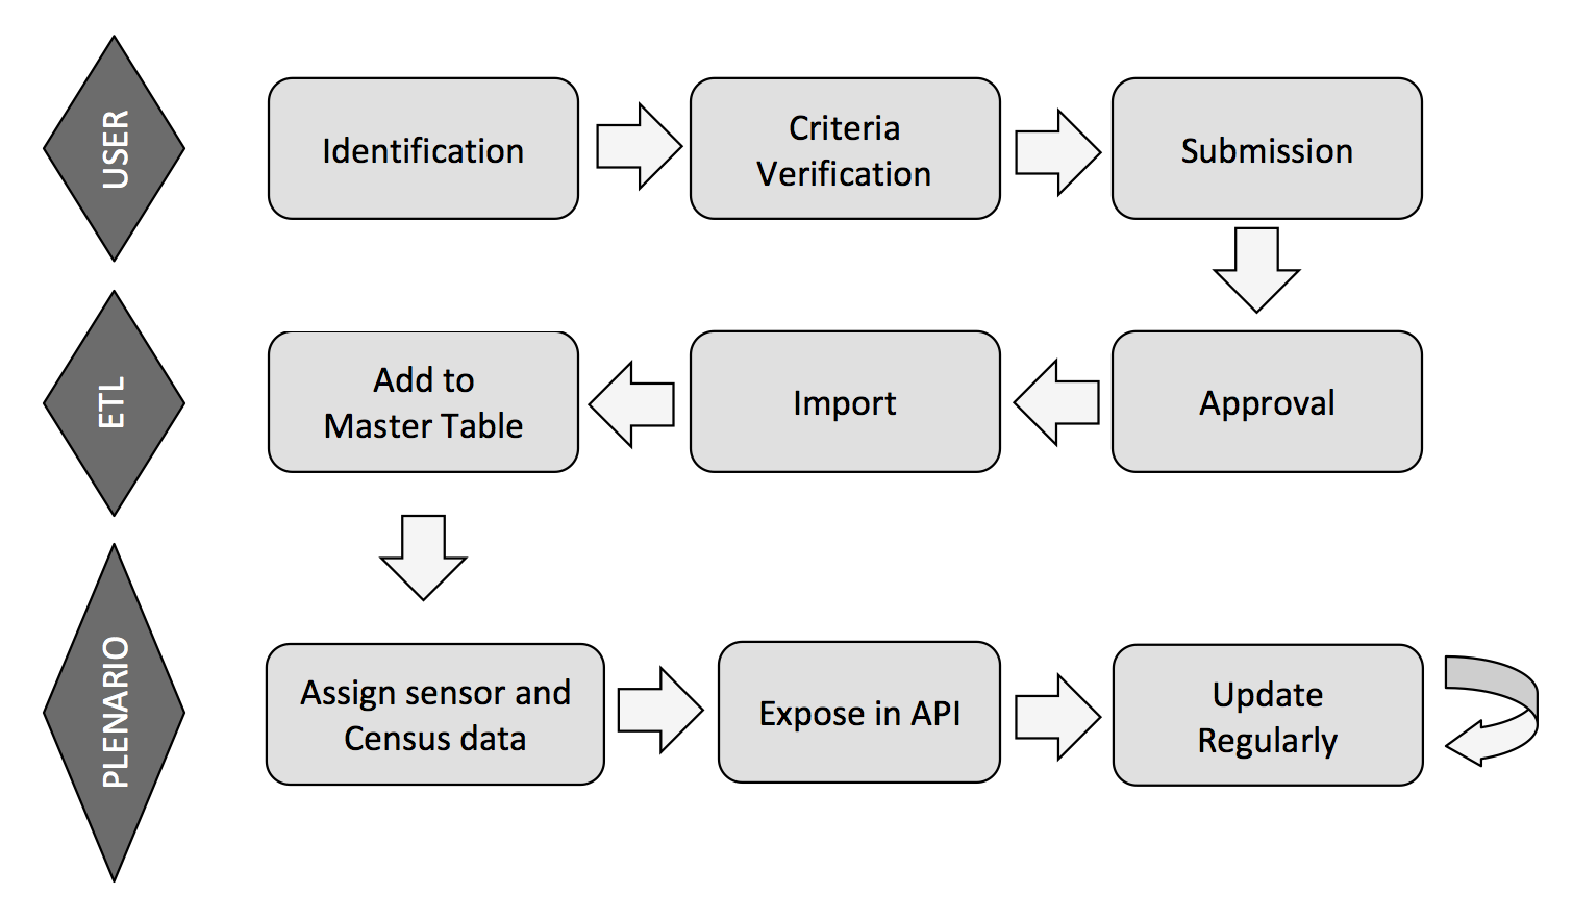
\includegraphics[width=0.8\textwidth]{flowchart}
\end{figure}

\subsection{Automated ETL Builder}

\subsection{Single Spatio-Temporal Index}

\begin{figure}[h]
	\caption{An example search using the user interface}
	\centering
	\includegraphics[width=0.8\textwidth]{search}
\end{figure}
\subsection{Sensor and Local Data}

\begin{figure}[h]
	\caption{PostgreSQL Schema}
	\centering
	\includegraphics[width=0.8\textwidth]{schema}
\end{figure}


\subsection{API Endpoints}
\section{Architecture}

\begin{figure}[h]
	\caption{Amazon Web Services Setup}
	\centering
	\includegraphics[width=0.8\textwidth]{aws}
\end{figure}


\section{Early Applications}

\section{Issues Encountered}

\subsection{Data Issues}

\subsection{Scaling Issues}

\subsection{Philosophical Issues}

\section{Conclusion}








\end{document}